\documentclass[../main.tex]{subfiles}
\graphicspath{{\subfix{../IMAGES/}}}

\begin{document}
\localtableofcontents

\subsection{Introduction}
Daily needs of an adult : 6-8MJ, 1 liter of oil : 36MJ, 100km in a car : 230MJ (6.4L).\\
A computer needs : 100-200W, a cyclist : 450W, an adult : 100W, car engine : 75kW (100hp).\\

The energy used is not the energy harvested : energy resources (primary : contained in raw fuels before the start of the conversion chain) and energy services (final : received by consumers and businesses after energy losses in the conversion and distribution).\\

\begin{figure}[hbt!]
    \centering
    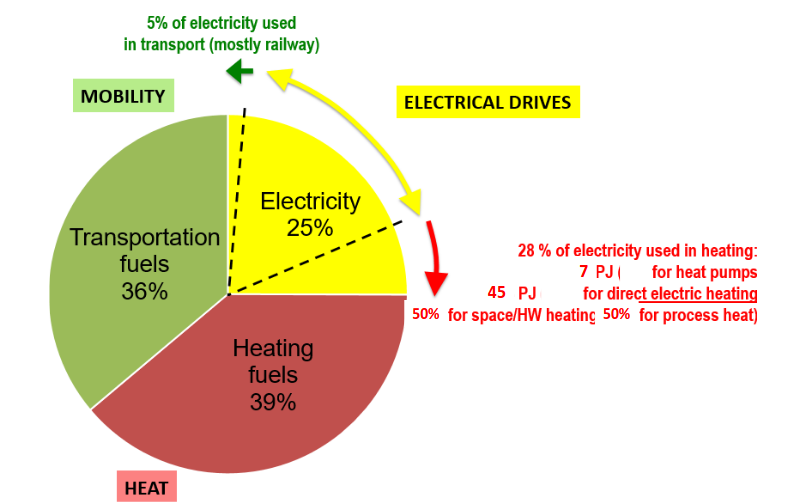
\includegraphics[width=0.6\linewidth]{IMAGES/Renewable/Screenshot from 2025-02-22 19-57-45.png}
\end{figure}

There are 6 energy and services : cooling, space heat, sanitary hot water, process heat, electricity and mobility. \\
\textbf{Energy reserves} are proven and valid for current production rates at present economics. \textbf{Ultimate reserves} (physical) are multiple times larger, recoverable at higher cost, extending the use to several centuries. \\

Main drivers for the rise in energy demand : demographic growth, improvement of standard of living and intensity of energy service. 

Classification wrt timescale : instantaneous (seconds/minutes : solar, wind, hydro), short term storage (days/week : wind, hydro, waves, tides), medium term storage (months/years : biomass, wastes, geothermal), long term storage (millions of years : oil, gas, coal, nuclear, geothermal).\\
Essential needs are : food (biomass), cheap abundant energy, clean water, clean air, health care, waste management, education...\\

\warning The molar mass of a system can be computed as : \begin{equation}
\begin{gathered}
    M = \frac{R}{c_p \frac{\kappa-1}{\kappa}} = \frac{8.314}{c_p \frac{\kappa-1}{\kappa}}
    \frac{T_a}{T_b} = (\frac{p_b}{p_a})^{\frac{\kappa-1}{\kappa}}\\
    pv^\kappa = cte
\end{gathered}
\end{equation}
with $R = 8.314 J\cdot mol^{-1} K^{-1}$.\\

\subsection{Thermodynamics}
[Time rate of change of the energy contained within the control volume at time t] = [net rate of energy transferred in across system boundary by heat transfer at time t] - [net rate of energy transferred out across system boundary by work transfer at time t] + [net rate of energy transferred out across system boundary by work transfer at time t]\\
$\Delta E = \Delta U + \Delta PE + \Delta KE = Q-W+E_{in}-E_{out}$\\

Energy conservation : $\frac{dE_{cv}}{dt} = \dot{Q}-\dot{W} + \sum_i \dot{m}_i (h_i + \frac{w_i^2}{2} + gz_i) - \sum_e \dot{m}_e (h_3 + \frac{w_e^2}{2}+gz_e)$.\\
In a nozzle/diffusor : $h_i+\frac{w_i^2}{2} = h_e+\frac{w_e^2}{2}$ (total enthalpy is conserved).\\
In throttling valves : $h_i=h_e$.\\
In a turbine, compressor, pump, fan : $0=-\dot{W} + \dot{m}(h_i + \frac{w_i^2}{2} + gz_i)-\dot{m}(h_e + \frac{w_e^2}{2} + gz_e)$.\\
In a heat exchanger : $0 = \sum_i \dot{m}_i h_i - \sum_e \dot{m}_e h_e$.\\

Combustion efficiency : $\eta_{comb} = \frac{\dot{Q}}{\dot{m}HV}$, with HV the heating values, HHV if water is condensed, LHV if water exhaust remains vapor (cars, jet engines ...).\\
\begin{table}[hbt!]
    \centering
    \begin{tabular}{c|c|c}
    Fuel & HHV [MJ/kg] & LHV [MJ/kg] \\ \hline
    $H_2$ & 141.8 & 119.96\\
    $CH_4$ & 55.5 & 50\\
    Ethane & 51.9 & 47.8\\
    Propane & 50.35 & 46.35\\
    Butane & 49.5 & 45.75\\
    Gasoline & 47.3 & 44.4\\
    Kerosene & 46.2 & 43\\
    Diesel & 44.8 & 43.4\\
    Coal (anthracite) & 32.5 & \\
    Coal (lignite) & 15 & \\
    Wood & 21.7 & 20\\
    \end{tabular}
\end{table}

A cycle is a series of processes that return a system to its initial state : $\Delta E = 0 = Q_{cycle} - W_{cycle}$. Power cycle : $\eta_{th} = \frac{W_{cycle}}{Q_{cycle}} = 1-\frac{\lvert Q_{out}\rvert}{Q_{in}}$ (carnot). Refrigeration and heat pump : $COP_{c} = \frac{Q_{in}}{\lvert W_{cycle} \rvert} = \frac{Q_{in}}{\lvert Q_{out} \rvert - Q_{in}}$, $COP_h = \frac{Q_{out}}{W_{cycle}} = 1+COP_c$.\\

In general : $\Delta S = \int \frac{\delta Q}{T}+\sigma$, if reversible $\sigma = 0$. \warning In closed system! Otherwise : $\frac{dS}{dt} = \sum \frac{\dot{Q}_j}{T_j} + \sum_i \dot{m}_i s_i - \sum_e \dot{m}_e s_e + \dot{\sigma}$.\\

Isentropic efficiencies (turbine) : $\eta_{t,s} = \frac{h_1-h_2}{h_1-h_{2,s}}$, (compressor) : $\eta_{c,s} = \frac{\Delta h_{s,1-4}}{\Delta h_{1-4}}$.\\

\quad \underline{Carnot cycle :}\\
Cycle that undergoes four reversible processes. Two isothermal processes at two different temperature. Two isentropic processes. Clockwise : work cycle, anti-clockwise : heat pump/refrigeration.\\
\begin{table}[hbt!]
    \centering
    \begin{tabular}{c|c|c|c}
     & Work cycle & Heat cycle (refrigeration) & HC (heat pump)\\ \hline
    Efficiency & $\eta = 1-\frac{Q_c}{Q_h}$ & $COP_c = \frac{Q_c}{Q_h-Q_c}$ & $COP_h = \frac{Q_h}{Q_h-Q_c}$ \\ \hline
    Max. efficiency & $\eta_{max} = 1-\frac{T_c}{T_h}$ & $COP_{c,max} = \frac{T_c}{T_h-T_c}$ & $COP_{h,max} = \frac{T_h}{T_h-T_c}$\\
    \end{tabular}
\end{table}

\quad \underline{Exergy :}\\
It is defined as : $Ex = U-U_0 + KE + PE - T_0(S-S_0) + p_0(V-V_0)$.\\
Exergy efficiency expresses the work-equivalent efficiency of energy resource utilization : $\varepsilon_{ex} = \frac{\text{used exergy}}{\text{provided exergy}}$.\\
\begin{itemize}
    \item Turbine : $\varepsilon_{ex} = \frac{\dot{W}}{\dot{m}(ex_{f,i} - ex_{f,e})}$
    \item Compressor/pump : $\varepsilon_{ex} = \frac{\dot{m}(ex_{f,e} - ex_{f,i})}{-\dot{W_{cv}}}$
    \item Heat exchanger : $\varepsilon_{em} = \frac{m_c (ex_{f,e,c} - ex_{f,i,c})}{m_h (ex_{f,i,h} - ex_{f,e,h})}$
\end{itemize}

In a turbine, the exergy losses are : $\dot{L} = T_a(\sum_{i, leaving} \dot{M}_is_i - \sum_{j, entering} \dot{M}_j s_j) + \dot{Q}_a^-$, caused by the dissipation in the steam network. \\
The exergy losses in a compressor are : $\dot{L} = T_a \sum_j s_j \dot{M}_j^-$.\\
In both cases, the efficiency is : $\eta=1-\frac{\dot{L}}{\dot{E}^+}$.\\

In vapor power systems, the ideal efficiency is : $\eta_{ideal}= 1-\frac{T_{out}}{\overline{T}_{in}}$.\\
In a rankine cycle, improving performance can be done via : superheating (additional heat exchanger), reheating, regeneration (feedwater heater).\\

\quad \underline{Internal combustion engines :}\\

\begin{itemize}
    \item Air-standard Otto cycle : \begin{figure}[hbt!]
        \centering
        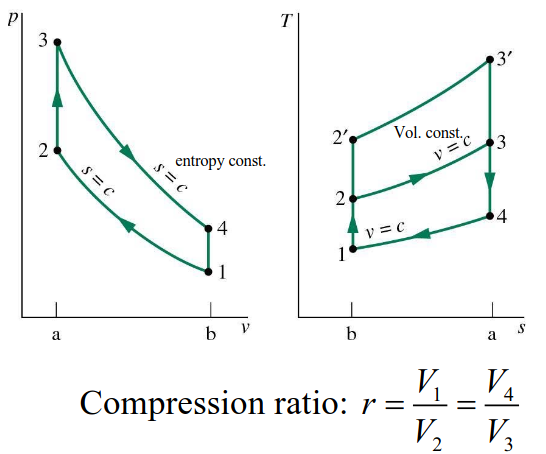
\includegraphics[width=0.5\linewidth]{IMAGES/Renewable/Screenshot from 2025-02-25 21-57-41.png}
    \end{figure}
    1-2 : isentropic compression ($W = m(u_1-u_2)$), 2-3 : constant volume heat transfer ($Q = m(u_3-u_2)$), 3-4 : isentropic expansion ($W = m(u_3-u_4)$), 4-1 : constant volume heat rejection ($Q = m(u_1-u_4)$). Efficiency : $\eta = \frac{u_3-u_4+u_1-u_2}{u_3-u_2}$.
    \item Air-standard diesel cycle : \begin{figure}[hbt!]
        \centering
        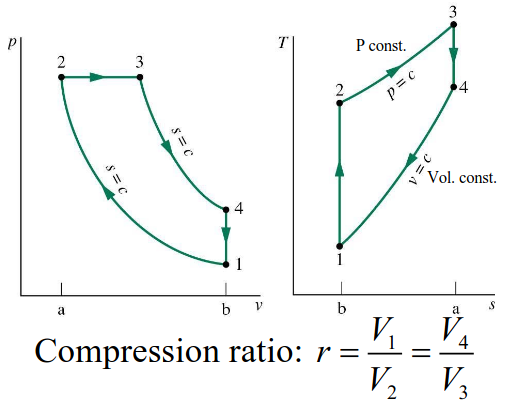
\includegraphics[width=0.5\linewidth]{IMAGES/Renewable/Screenshot from 2025-02-25 22-00-44.png}
    \end{figure}
    1-2 : isentropic compression ($W = m(u_1-u_2)$), 2-3 : constant pressure heat transfer ($W = mp_2(v_3-v_2)$, $Q = mW + m(u_3-u_2)$), 3-4 : isentropic expansion ($W = m(u_3-u_4)$), 4-1 : constant volume heat rejection ($Q = m(u_1-u_4)$). Efficiency : $\eta = \frac{h_3-h_2-u_4+u_1}{h_3-h_2}$.
    \item Air-standard Brayton cycle (gas turbine) : \begin{figure}[hbt!]
        \centering
        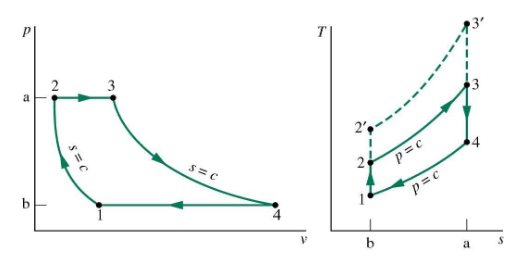
\includegraphics[width=0.5\linewidth]{IMAGES/Renewable/Screenshot from 2025-02-25 22-04-31.png}
    \end{figure}
    1-2 : isentropic compression, 2-3 : isobaric heat transfer, 3-4 : isentropic expansion, 4-1 : isobaric heat transfer. Efficiency : $\eta = \frac{h_3-h_4+h_1-h_2}{h_3-h_2}$. Performance increases with pressure ration. Can also be improved with intercooling, regeneration, reheating. 
\end{itemize}

\quad \underline{Combined cycle :}\\
Gas cycle (Brayton) on top of steam cycle (Rankine). Gas turbine reduces exergy heat transfer loss while steam turbine reduces heat exergy loss. \\

\begin{figure}[hbt!]
    \centering
    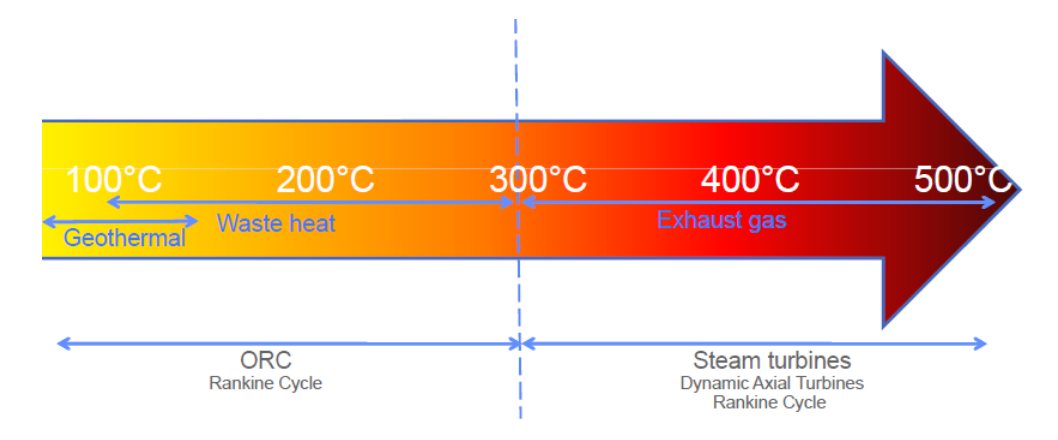
\includegraphics[width=0.8\linewidth]{IMAGES/Renewable/Screenshot from 2025-02-26 00-40-53.png}
\end{figure}

\subsection{Geothermal energy}
Average gradient of $30K/km$ in the crust. 

\begin{figure}[hbt!]
    \centering
    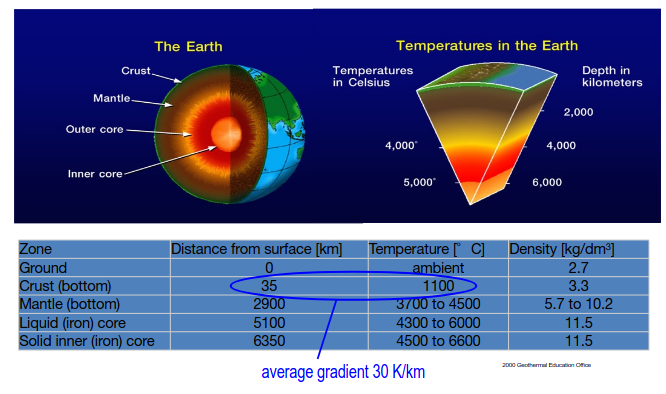
\includegraphics[width=0.5\linewidth]{IMAGES/Renewable/Screenshot from 2025-03-04 21-24-14.png}
\end{figure}

In volcanic activity : $100K/km$ with heat flux $1-3W/m^2$. In tectonic activity : $50K/km$ with heat flux $0.1W/m^2$, in local anomalies : $40K/km$ with heat flux $0.07W/m^2$, in continental mean $30K/km$ with heat flux $0.05W/m^2$.\\

The average goethermal heat flux is around $50-60mW/m^2$ resulting from the flux from hot earth interior and radioactive decay within the crust.\\
This corresponds to $6.75TW_{heat}$ (assuming $20\%$ electrical efficiency and 8000h load : $1.35TW_{el}$ and $11000TWh_{el}$ which is $40\%$ of the current world electrical production).\\

In reality : $15GW_{el}$ ($85TWh_{el}$) supplied worldwide. \\

\warning It can be unsustainable! If heat extraction rate > geothermal heat flux then the soil is cooled down. \\
It can serve as a baseload power, considered as free fuel but the drilling is expensive. \\
Geothermal systems are related to young igneous rock (one of the 3 main rock types formed through the cooling and solidification of magma/lava) intrusions in the upper earth crust. HDR (hot dry rock) and convective hydrothermal reservoirs are exploited in geothermal PP.\\

\begin{table}[hbt!]
    \centering
    \begin{tabular}{c|c|c|c}
        Characteristic & Temperature & Depth/Location & Plant type \\ \hline
        Low T water & 100-150$^\circ C$ & <3km, gradient of $50K/km$ & binary, ORC\\
        High T water & 150-370$^\circ C$ & <2km, gradient > $100K/km$ & Flash \\
        Vapor & >$200^\circ C$ & <2km & Dry steam\\
    \end{tabular}
    \caption{Classification of hydrothermal reservoirs}
\end{table}

Electricity production potential : hot source is the geothermal resource and cold source is a river/ambient air. Maximum available power : $Ex = (1-\frac{T_0}{T_h})\dot{Q}_{in}$. The efficiency : $\eta = \frac{\dot{W}_{cycle}}{\dot{Q}_{in}}$ (energy quantity) and the exergy efficiency : $\varepsilon = \frac{\dot{W}_{cycle}}{(1-\frac{T_0}{T_h}) \dot{Q}_{in}}$ (energy quality).\\

The \textbf{Logarithmic mean temperature difference} of heat exchanger : $LMTD = \frac{(T_{h1}-T_{c1})- (T_{h2}-T_{c2})}{\ln(\frac{T_{h1}-T_{c1}}{T_{h2}-T_{c2}})}$ and the transferred heat : $Q = U\cdot A \cdot LMTD$.\\
This is a heat exchange between a hot fluid cooling from $T_{h1}$ to $T_{h2}$ and a cold fluid warming from $T_{c1}$ to $T_{c2}$.\\

As the geothermal reservoir is not a constant temperature source one has to average $T_h$ is : $LMT = \frac{T_{h,in}-T_{h,out}}{\ln(\frac{T_{h,in}}{T_{h,out}})}$.\\

\subsubsection{Dry steam PP}
Steam shoots up the wells directly into a turbine. They are rare.\\

\subsubsection{Flash steam plant}
Flash technology was invented in New Zealand. They are common as most reservoirs are hot water reservoirs. \\
As hot water is released from the high pressure of the deep reservoir in a flash tank, some of it becomes steam. \\

\begin{figure}[hbt!]
    \centering
    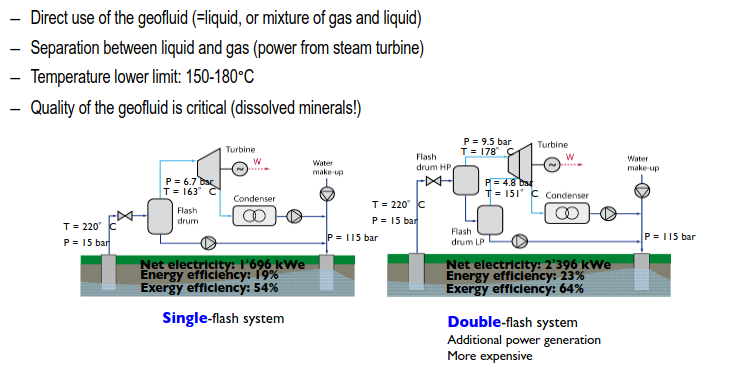
\includegraphics[width=0.5\linewidth]{IMAGES/Renewable/Screenshot from 2025-03-04 22-23-41.png}
    \caption{Flash conversion cycles}
\end{figure}

\subsubsection{Binary cycle PP}
Heat from the geothermal water is used to vaporize a working fluid in a 2nd network. This vapor powers the turbine. Temperature lower limit : $70-90^\circ C$. No emissions of geofluid to atmosphere. \\

To increase the electrical efficiency : flash system with bottoming ORC. Cogeneration increases energy and exergy efficiency due to the use of waste heat. \\

HDR corresponds to Hot Dry Rock and DHM Deep Heat Mining but is unsustainable.\\

\subsubsection{Geothermal heat for buildings}
2 heat demands in buildings : hot sanitary water, space heating. Around \textbf{50L/day/person} at $50^\circ C$ hot source and $10^\circ C$ cold source. ($\dot{Q} = \dot{m}c_p \Delta T = 2.32 \frac{kWh}{day} = 100W$.\\

Space heating requirement : loss (compensate for $\Delta T = T_{in}-T_{out}$), gains (any internal heat sources). Energy balance = LOSSES-GAINS = $\eta_{system} E_{heating_system} = P_{system} t$.\\

\quad \underline{Conduction losses : }\\
\begin{equation}
    \dot{Q} = A [m^2] U [\frac{W}{m^2 K}] \Delta T[K]
\end{equation}
With A the contact area (walls, windows, roof...), U the thermal conduction coefficient (floor against soil : 0.3, roof : 0.2, walls : 0.3, windows : 1.3, doors : 2), $R = \frac{1}{U}$ the thermal resistance coefficient. \warning If multiple layers : $R_{tot} = \sum R_i$.\\

\quad \underline{Convection losses : }\\
\begin{equation}
    \dot{Q} = V[m^3] N [s^{-1}] C_p [\frac{J}{m^3 K}] \Delta T [K]
\end{equation}
With : $C_p = 1200 J/m^3L$ for air ($1kJ/kgK$ and $1.2 kg/m^3$), N the air replacement number via leaks (for example one person requires $30m^3/h$ of air replacement.\\

One rule of thumb : total losses are $1\frac{W}{m^2 K}$. (If the house is $200m^2$ : total losses are $207W/K  = 5 \frac{kWh}{dayK}$\\

\quad \underline{Degree-days (DD) :}\\
Energy loss(J) = loss-coefficient (W/K) x $\Delta T$x time (s) : $\Delta T$x time = Degree days (temperature demand, i.e. $T_{in} = 20^\circ C$, $T_{out} = 10^\circ C$ for 1 week is $70 DD$).\\

A typical year number for Switzerland is 3000DD (with $\Delta T = 8^\circ C$). Which gives an energy loss : $E(j) = 207*3000*24*3600 = 54GJ = 14900kWh$ or $270 MJ/m^2yr$.\\

\quad \underline{Gains :}\\
People emit power (100W per adult, 60W for children) as well as the house ($2W/m^2$). \\

A reduction by a factor of 4 between current consumption and future construction standards is realistic.\\
\warning Occupant behaviour has a significant impact on the consumption.\\


\quad \underline{Dynamic behaviour - heat diffusion 1st law :}\\
\begin{equation}
    Q = -\lambda \frac{dT}{dx}
\end{equation}
With $\lambda [\frac{W}{mK}] = \rho C_p [\frac{J}{kg K}] D[\frac{m^2}{s}] = C_v [\frac{J}{m^3K}] D[\frac{m^2}{s}] = U d[m]$, $\lambda$ the thermal conductivity, U the thermal conduction coefficient, d the thickness of the material, C the heat capacity of the material, D the heat diffusion coefficient. 

\begin{figure}[hbt!]
    \centering
    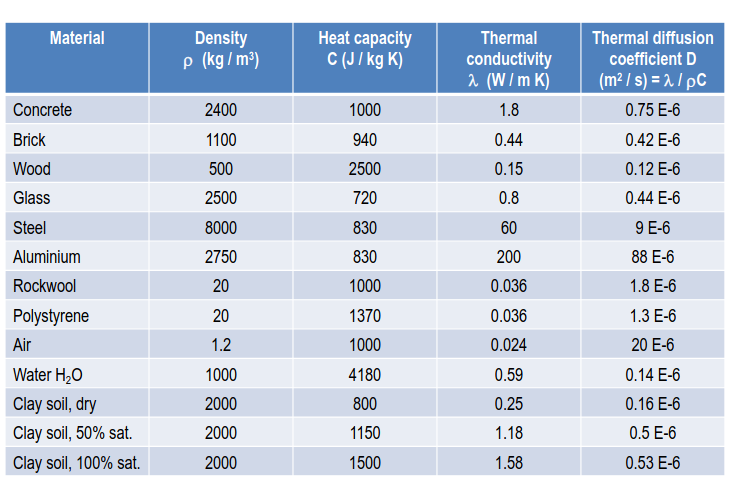
\includegraphics[width=0.5\linewidth]{IMAGES/Renewable/Screenshot from 2025-03-11 20-18-18.png}
    \caption{Materials thermal properties}
\end{figure}

The distribution is given by : $\frac{dT}{dt} = D \frac{d^2 T}{dx^2}$ in 1D, with the solution : $T = \frac{K}{\sqrt{t}} \exp[-\frac{x^2}{4Dt}]$, with the integration constant K : (computation of $Q = \int m CdT$)
\begin{equation}
    \begin{gathered}
        K = \frac{Q}{2\rho C \sqrt{\pi D}} = \frac{Q}{2\sqrt{\pi \rho C \lambda}}\\
        T(x,t) = \frac{Q}{2\rho C \sqrt{\pi Dt}} e^{-\frac{x^2}{4Dt}}
    \end{gathered}
\end{equation}
With $\sqrt{Dt}$ the characteristic length. \\

Assume a seasonal sinusoidal variation of temperature T at the ground surface : $T(0,t) = T_{surface} = T_{avg} + A\cos(\frac{2\pi}{T_{period}}t)$. One solution is : $T(x,t) = T_{x,soil depth} = T_{avg} + Ae^{-\frac{x}{x_L}}\cos(\frac{2\pi}{T_{period}} t - \frac{x}{x_L})$ with $x_L = \sqrt{\frac{DT}{\pi}}$ the characteristic depth (m) of both the decay and oscillation. \\
The resulting heat flux is then : $Q(x) = -\lambda \frac{dT}{dx} \frac{A}{x_L} e^{-\frac{x}{x_L}} \sqrt{2} \sin(\frac{2\pi}{T_{period}}t - \frac{x}{x_L} - \frac{\pi}{4})$ and the peak flux at the surface : $Q(0) = \lambda \frac{A}{x_L}\sqrt{2} = A\sqrt{\frac{2\pi}{T}} \sqrt{\lambda \rho C}$.\\


\subsection{Solar energy}
Solar power constant on ground level is around $1kW/m^2$. Depending on the location : $2-10kWh/m^2day$ or $1000-2000 kWh/m^2 year$.\\

Fusion reactions inside a star : proton-proton cycle (pp), the most important and carbon-nitrogen oxygen cycle (CNO). The reaction sequence requires 4 protons summarized by : $4 {}_1^1H \rightarrow {}_2^4 H_e + 2e^+ + 26.73MeV = 4.29$ ($4.29\cdot 10^{-12}J$).\\
$0.712\%$ of H-mass becomes energy such that $6\cdot 10^{11} kg/s$ H transformed into $H_e$.\\
The sun's radiation is : $E= \sigma T^4 = 63 MW/m^2$ ($\sigma = 5.67 \cdot 10^{-8} W/m^2K^4$ and $T_{sun} = 5780K$) while on Earth we receive : $E = 1368 \pm 1W/m^2$.\\
The annual variation in radiation : \begin{equation}
    I_{day} = I_0 (1+0.033 \cos[2\pi (\frac{day}{365})]) \: [W/m^2]
\end{equation}
In general it goes between $\pm 3.3\%$.\\

Sun spots are colder and appear with a 11 year periodicity. Solar radiation intensity changes may be $1\%$. Power variation per surface unit is : $\frac{dE}{dT} = 4\sigma T^3 = 43.8\cdot 10^3 W/m^2K$.\\
For $\Delta T=1K$, power variation is $0.07\%$ of the real value, this changes the solar constant by $1W/m^2$!\\

The energy received by the Earth in one year is : $175PW$, which is 9000 times the present human annual energy need. The mean solar irradiance onto earth's atmosphere is divided by 4 : $342W/m^2$ (with Earth's albedo taken into account $236W/m^2$). Assuming $20\%$ efficient PV 0.1\% of earth surface is needed to deliver global annual energy. Global annual energy need delivered in 1h. \\

Reflected back to space by albedo : $31\% \Rightarrow 3.85\cdot 10^{24} J/yr$ intercepted.\\
\warning Taking into account albedo, only $943W/m^2$ is received at Earth's surface.\\

What matters is the annual solar energy input on a given location (P). This depends on the latitude $\phi$ of point P which in turn determines the seasonal variation (declination $\delta$), the orientation of the receiver surface at point P w.r.t. the Sun's height (zenith $\xi$) and the south, the daily weather conditions.\\
Solar declination is defined as the angle between the equator plane and the line joining the center of the Earth to the center of the Sun : $\delta = 23.45^\circ \sin(2\pi \frac{284+J}{365})$.\\

Solar input on horizontal surface needs correction due to the sun's height (difference to zenith) : $\dot{E} = SI_0 (\frac{\overline{r}}{r})^2 \cos \xi [W]$, with $I_0$ the solar constant, $S$ the area of receiving surface, r the instantaneous Earth-sun distance, $\overline{r}$ the mean Earth-sun distance, $\xi$ the incident angle made by the solar radiation with the vertical of the receiving surface S : $(\frac{\overline{r}}{r})^2 \simeq (1+0.033\cos[2\pi \frac{day}{365}])$.\\

The solar hour angle H at point M is zero at midday ($H_{D/2}$ is the hour of sunrise [rad]). Day duration D[h] at latitude $\phi$ when declination is $\delta$ : $\cos \xi = \sin \phi \sin \delta + \cos \phi \cos \delta \cos H$, $H_{D/2} = \arccos(-\tan \phi \tan \delta)$ and $D = \frac{2 H_{D/2}^\circ}{15^\circ/h}$.\\

Energy received in one hour on a horizontal surface S is : $E_{hour} = 3600 S I_0 (\frac{\overline{r}}{r})^2 \cos \xi$. The energy received from sunrise to sunset on that surface : $E_{day} = \int_{-H_{D/2}}^{H_{D/2}} \frac{E_{hour}}{\pi/12} dH = \frac{24}{\pi} 3600 S I_0 (\frac{\overline{r}}{r})^2 \sin\phi \sin \delta [H_{D/2} (\frac{\pi}{180}) - \tan H_{D/2}] = 10.45 A(albedo)(\frac{\overline{r}}{r})^2 \sin\phi \sin \delta [H_{D/2} (\frac{\pi}{180}) - \tan H_{D/2}] \: [kWh/m^2]$.\\

\begin{figure}[hbt!]
    \centering
    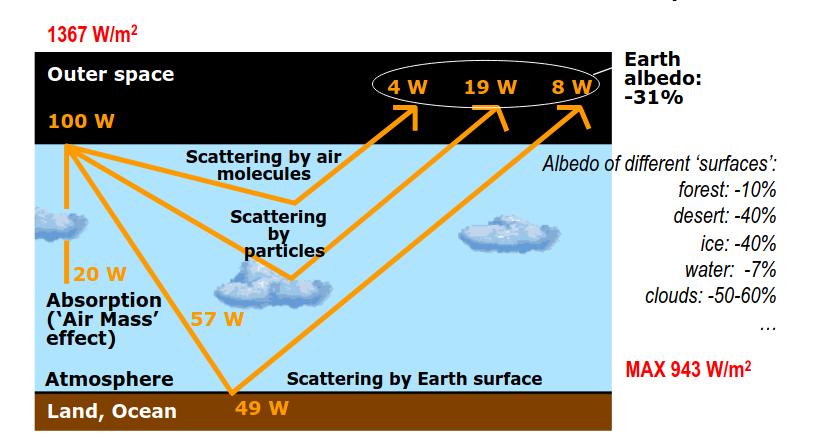
\includegraphics[width=0.5\linewidth]{IMAGES/Renewable/Screenshot from 2025-03-18 21-43-31.png}
\end{figure}

\begin{itemize}
    \item Diffusion scattering : different types of scattering occur according to the relative sizes of the scattering targets compared to the wavelength of the incident radiation. 
    \item Absorption : certain atmospheric molecules (ozone, $CO_2$ and $H_2O$) absorb the energy of various wavelength. AM (air mass) is the effective atmosphere thickness the sunrays have to travel between the sun's height position Z and an observer on ground at 100m a.s.l. : $AM = \frac{P[mbar]}{1000} \frac{1}{\sin Z}$ 
\end{itemize}

Due to these interactions, the solar energy falling on the surface is significantly less than the extraterrestrial one ($1367W/m^2$). It is reduced on average to $49\%$ by scattering and absorption in the atmosphere and by daily weather conditions.\\

Planck's law of radiation : $I(\lambda) = \frac{2hc^2/\lambda^5}{\exp(\frac{hc}{\lambda kT}) -1} [W/m^3]$, with $h = 6.62\cdot 10^{-34}Js$, $k = 1.38\cdot10^{-23}J/K$ and $c=2.9979\cdot 10^8 m/s$.\\

We distinguish 3 processes : solar radiation ($0.2-4\mu m$ short waves, entering the atmosphere is absorbed and scattered back to space befor reaching the ground), thermal radiation (long wave $4-100\mu m$ from the heated surface of the earth and the atmosphere above, this amounts to $16\%$ of the total solar radiation being re-emitted as long wave radiation), non-radiative (heat and energy transport processes in the atmosphere and between soil/ocean and the atmosphere make up the remaining $33\%$ of the total in the balance).\\

\begin{figure}[hbt!]
    \centering
    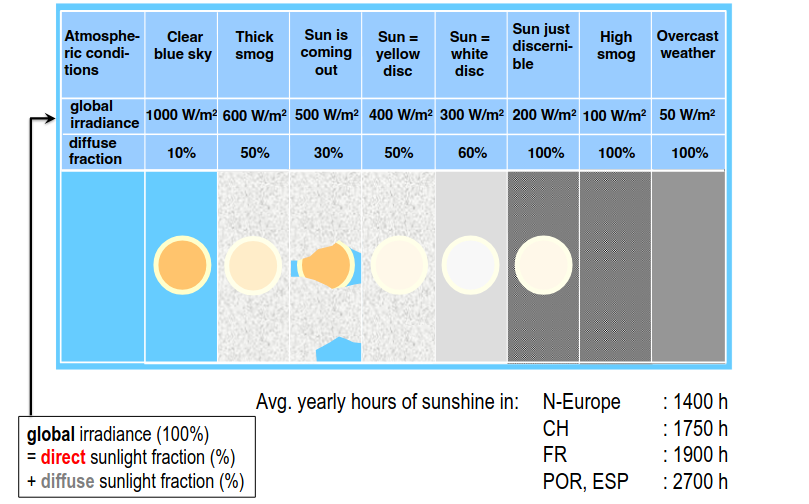
\includegraphics[width=0.5\linewidth]{IMAGES/Renewable/Screenshot from 2025-03-18 22-35-38.png}
\end{figure}

\subsection{Solar thermal technologies}
Passive systems capture heat through building design. Active systems are PV or thermal collector surfaces. \\
Unconcentrated solar thermal collection (direct+diffuse), $33\%$ capture loss, $2\%$ pipe losses, $25\%$ unused summer excess so we go from $1200kWh/m^2 yr$ as input to $400kWh/m^2yr$ which means we need around $2m^2$ of collector area/person. \\
Efficiency of flat solar collector : $E_{eff} = E_{in}-(E_{refl} + E_{front} + E_{rear})$. To limit the losses : operator collector at low T, reduce the absorber surface, good insulation, front glazing, selective coating on absorber, vacuum. $\eta = \frac{\dot{E}_{eff}}{\dot{E}_{in}} = A_0 - K \frac{\Delta T}{\dot{E}_{in}} = A_0 - Kx$, $A_0$ the absorption coefficient, $K$ the conduction/convection loss coefficient ($W/m^2K$).\\

\quad \underline{Concentrating solar power plants (CSP) :}\\
CSP plants concentrate the solar energy (direct only) using mirrors into high temperature heat which generates power via gas/steam turbines. Three types : parabolic trough (line concentration, $300-400^\circ C$, c=50, lowest cost), parabolic dish (point concentration, $750^\circ C$, 7 to 25 kWe, c=2000, use of stirling engine or brayton cycle), central receiver (point concentration, $565^\circ C$, c=500, sun-tracking mirrors : heliostats).\\

\begin{figure}[hbt!]
    \centering
    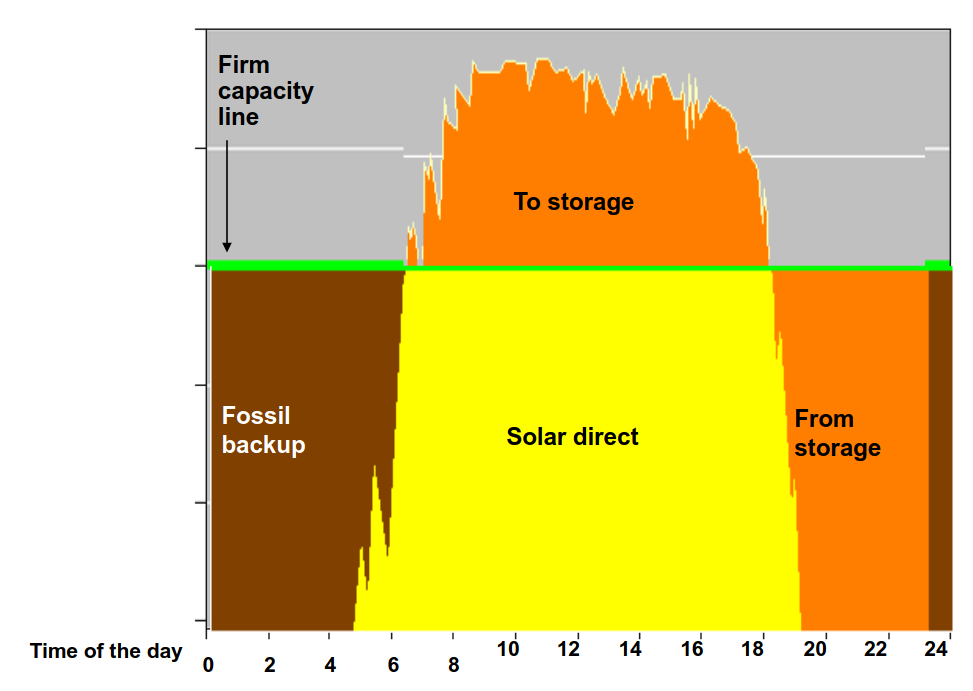
\includegraphics[width=0.5\linewidth]{IMAGES/Renewable/Screenshot from 2025-03-25 22-50-58.png}
\end{figure}

For a typical field : $22500$€/heliostats (for 1000 units produced). \\
Typical losses : available global irradiation ($124\%$), available direct irradiation ($100\%$), plant availability ($78\%$), collection efficiency ($56\%$), radiatio2heat conversion ($42\%$), heat transport \& storage losses in cycle ($38\%$), thermodynamic \& electromechanical conversion ($18\%$), plant parasitic losses ($17\%$). Net final output : $\mathbf{17\%}$.\\

\begin{figure}[hbt!]
    \centering
    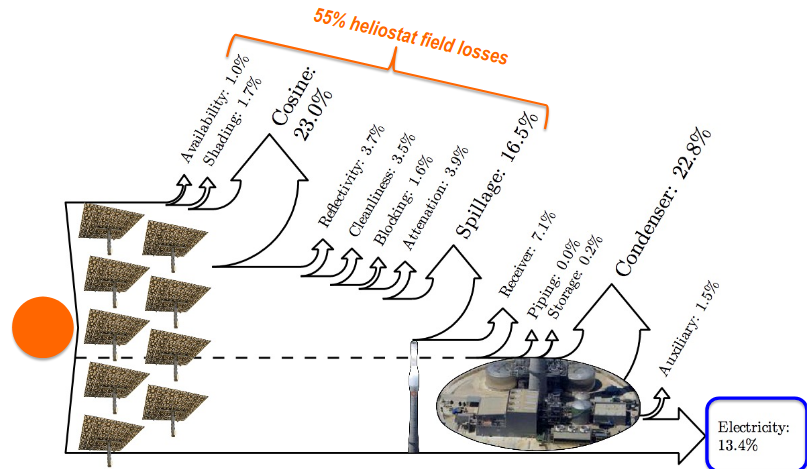
\includegraphics[width=0.7\linewidth]{IMAGES/Renewable/Screenshot from 2025-03-25 23-03-56.png}
\end{figure}
Capacity factor is around $0.64$ (5600h). An optimum LCOE can be found to be $24cts/kWh_{el}$ for a payback time of 10 years ($8850 $€$/kWe \simeq 150$M€). Decision variables are heliostat width, heliostat height, radial spacing, south to north ratio, number of heliostats, aim height, receiver height, receiver width.\\
Multi-tower plants improve the performance (annual field efficiency) but increases the LCOE.\\

\subsection{Photovoltaics (solar cells)}
It relies on direct conversion : of incident energy of photons on a SC, into electricity by the creation of pairs of charge carriers in the SC, and the separation of these thanks to a p-n junction. In atoms, electrons are found on precise and confined energy levels (orbitals). When closely arranging many identical atoms in a solid, these energy levels combine to form continuous energy bands between 2 energy values : filled (shell electrons), partially filled (valence electrons) and empty (allowed energy levels but without electrons).\\
The Fermi distribution describes how to fill these energy levels. The density of authorized energy levels for the electrons in the confined crystal volume is given by the Fermi distribution. Number dN of electrons in the energy level interval E+dE : $dN = N_0 f(E)dE$ with $f(E) = \frac{1}{1+e^{\frac{E-E_F}{kT}}}$ with $N_0$ the total number of electrons. \\
\textbf{Fermi energy level :} highest occupied level by electrons (most weakly bounded to the nuclei).\\

For a SC, the Fermi level $E_F$ is located between 2 bands. Above : conduction band, below : valence band.\\
Intrinsic SC : $E_F$ right at the middle of the bandgap.\\
n doped (Phosphor): $E_F$ is close to the conduction band.\\
p doped (Boron): $E_F$ is close to the valence band.\\
Doping a SC reduces the resistance of the material. \\

When irradiating a SC, photons with energy $E_{photon} \geq E_{bg}$ excite electrons from bv to bc and creates a charge carrier pair. Then : $\lambda[nm] e_{bg} [eV] = 1240$.\\

Band bending : junction between SC and metal. Exchange until both material have the same Fermi level. It is compensated by an internal field. A charged double layer develops with potential difference : $\Delta \phi = \phi_{Me}-\phi_{SC}$. From Poisson's equation : $\nabla \phi = \frac{d\phi^2}{dx^2} = -4\pi \frac{q}{\varepsilon_0}$. \\
Junction between two SC (p-n) : charge exchange occurs across both bands until equilibrium is reached. An internal field exists which opposes the natural charge flows of electrons and protons. $i_{tot} = i_{e,0} (1-\exp(-\frac{e_0V}{kT})) +i_{p,0}  (1+\exp(\frac{e_0V}{kT}))$.\\
Forward bias : conducting diode, $V_{applied}$ is positive between p and n, electrons from n are drawn into p. \\
Reverse bias : blocking diode.\\
For a diode : $i_{tot} = (i_{e,0} + i_{p,0}) (e^{\frac{e_0V}{kT}}-1) = i_{dark}$.\\
If it is illuminated, photon energy $h\nu$ promotes electrons from bv to bc across the band gap. Then $i_{tot} = i_{dark} - i_{photo}$. Electrical current created by light is opposite to the natural charge flow of the p-n diode. \\
Then, for $V_{appl} = 0$ $i_{dark} = 0$, $i_{tot} = -i_{photo} = i_{cc}$, the sc current depends on the irradiance IRR and the bandgap : $i_{cc} = S (\text{sensibility, mA/mW}) \times IRR \times surface$ ($IRR \simeq 50-100 mW/cm^2$). \\
For $i_{tot} = 0$ : $V_{oc} = \frac{kT}{e_0} \ln(1-\frac{i_{cc}}{i_0}) = V_T \ln(-\frac{i_{cc}}{i_0})$ (in general 0.7V).\\ 
With $k = 1.38\cdot 10^{-23}$ and $e_0 = 1.6\cdot 10^{-19}$. Also : $i_{max} = i_{cc} (1-\frac{V_T}{V_{oc}})$
The power is then given by : $P = V [i_{cc} - i_0(e^{\frac{e_0V}{kT}}-1)]$ and the Fill-Factor (FF) : $FF = \frac{P_{max}}{V_{oc} I_{cc}}$ with $V_{max} = V_{oc} + V_T \ln \frac{V_T}{V_{max}}$. Then : $FF = \frac{V_{max}}{V_{oc}} [1- \frac{\exp(\frac{V_{max}}{V_T})-1}{\exp(\frac{V_{oc}}{V_T})-1}]$ (0.7 in general).\\

Solar cell efficiency is then : $\eta = \frac{P_{max}}{irradiance [W/cm^2] \times surface} = \frac{P_{max}}{i_{cc}/sensibility[A/W]} = S \times FF \times V_{oc}$ (in general $20\%$).\\
Temperature : $\frac{dV}{dT} = -2mV/K$ (small effect on $i_{cc}$). 

Solar PV power plants : should be > 100kWp to benefit from an economy of scale. \\

Recombinations : mechanisms of destruction of charge carriers (losses), return of electrons from bc to bv (luminescence), SHR impurities and structural defects capture $e^-$ and $p^+$, effect Auger the recombination energy is transferred to a third particle as kinetic energy. Recombination rate : $\frac{1}{\tau_p}$ (n-type) and $\frac{1}{\tau_n}$ (p-type).\\


Silicon PV technology : >85\% of the market, $E_{bandgap} = 1.12eV$, poor infrared absorption (wafer must be thick). \\
\underline{Fabrication :} reduction of sand $SiO_2$ by carbon ($SiO_2 + C \rightarrow Si+CO_2$), chlorination, reduction of $SiHCl_3$ by $H_2$ (impurities does to 0.1ppb). \\
To make crystalline Si : fusion at $1440^\circ C$ and growth of a tube. \\

Cell fabrication : chemical surface attack to reduce the surface light reflexion, diffusion of phosphorous in the surface, screenprinting of aluminium on the back + fusion (creation of the $p^+$ layer), deposition of silver-glass on the front by screen printing, deposit of silver on the back, titanium vapor treatment on the front (for antireflection), plasma attack to remove $n^-$ edges. \\

Thin film technology : lower quality and efficiency but lower cost Si, short current path, non-saturated Si bonds. \\

Concentrated PV : small cells of high efficiency, only direct solar irradiation is used (30-50 suns). 

\subsection{Biomass}
Photosynthesis is described as : $6CO_2 + 6H_2O \rightarrow C_6H_{12} O_6 + 6O_2$.\\
The glucose synthesis : $\Delta G = 2862kJ/mol$. For one molecule ($CO_2$), we need 8 to 10 photons.\\
Theoretical efficiency with white light : $28.6\%$.

\warning Theoretical biomass potential is $\simeq 1000$ times the human primary energy need. 
Biomass is dilute energy storage and approximates the formula $CH_2O$. \\

Advantages : renewable, $100\%$ use of collected matter. Drawbacks : dispersed resource, seasonal production, low energy density.\\

Classification : \begin{itemize}
    \item aquatic : algae
    \item terrestrial : \begin{enumerate}
        \item vegetable oil plants
        \item sugar/starch crops
        \item herbaceous
        \item wood (lignocellulosic)
    \end{enumerate}
\end{itemize}
It can also be classified by water content : dry ($<15$wt\% humidity), humid (15-30wt\% $H_2O$), slurry (30-90wt\% $H_2O$), liquid (>90wt\% $H_2O$).\\
It can also be classified by human activity : natural (no interference), residual (organic waste streams), cultivated (active use of land).\\
It can also be classified by chemical nature : lignocellulosic ($19MJ/kg$), amylaceous (starch, $19MJ/kg$), sugarous ($39MJ/kg$), lipidic ($22MJ/kg$).\\

Cellulose is $40-80$wt\% in plants, $17.5MJ/kg$. Linear polymer of up to 10 000 glucose molecules $(C_6H_{10} O_5)_n$. Lignine is a complex aromatic polymer, 25-35wt\% in wood, 10-25\% in plants, $26.6MJ/kg$. Hemi-cellulose, shorter polymer. \\
\begin{equation}
    LHV = 43.6\times C - 0.31 MJ/kg
\end{equation}

\subsubsection{Wood conversion}
\begin{figure}[hbt!]
    \centering
    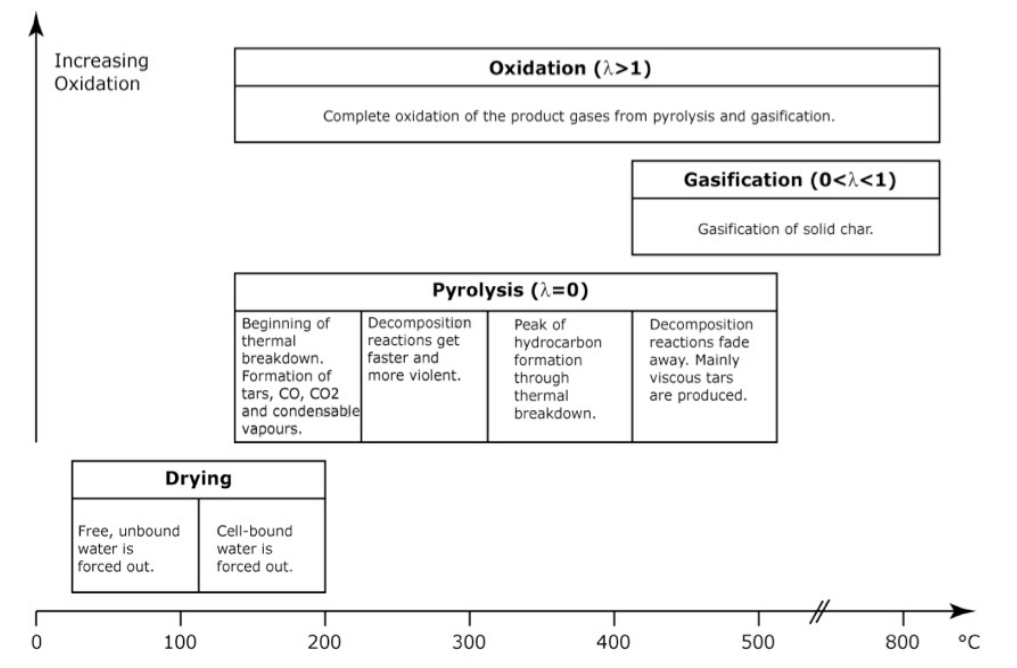
\includegraphics[width=0.5\linewidth]{IMAGES/Renewable/Screenshot from 2025-04-15 23-00-58.png}
    \caption{Combustion, gasification, pyrolysis, distinguished by the amount of oxygen addition $\lambda$.}
\end{figure}

Direct wood combustion : theoretical air-factor for dry wood is 6kg air/kg wood. The $LHV_{dry} = 17.46 \times C + 26.63 \times (1-C) \pm 0.4MJ/kg$, C the cellulose + hemicellulose and 1-C the lignine content. \\
$LHV_{humid} = LHV_{dry} \times (1-1.14W)$, W the water content in weight fraction. \\

\quad \underline{Pyrolisis :}\\
1000kg of wood generates 200kg of gas, 360kg of pyrolisis 'oil', 110kg of tars (condensable oxyhydrocarbons), 330kg of charcoal. \\

\quad \underline{Gasification :}\\
\begin{table}[hbt!]
    \centering
    \begin{tabular}{c|c|c|c}
        Process & Nature & Temperature range & Subproduct \\ \hline
        Drying & Endothermal & <$200^\circ C$ & dried biomass\\
        Devolatilisation (thermal decomposition without oxidant) & endothermal & 200-600 & $H_2, CO, CO_2, CH_4$, tars, charcoal\\
        Reducing & endothermal & 600-1000 & reforming, shift, methanation\\
        Oxidising & exothermal & 1000-1600 & $CO_2, H_2O$
    \end{tabular}
\end{table}

Updraft : air comes from the bottom of the tank and pellets are added. Because gases have to go through unburned pellets to exit, it contains less particles but produces lots of tars on the walls (low T). \\

\quad \underline{Impurities from wood :}\\
\begin{figure}[hbt!]
    \centering
    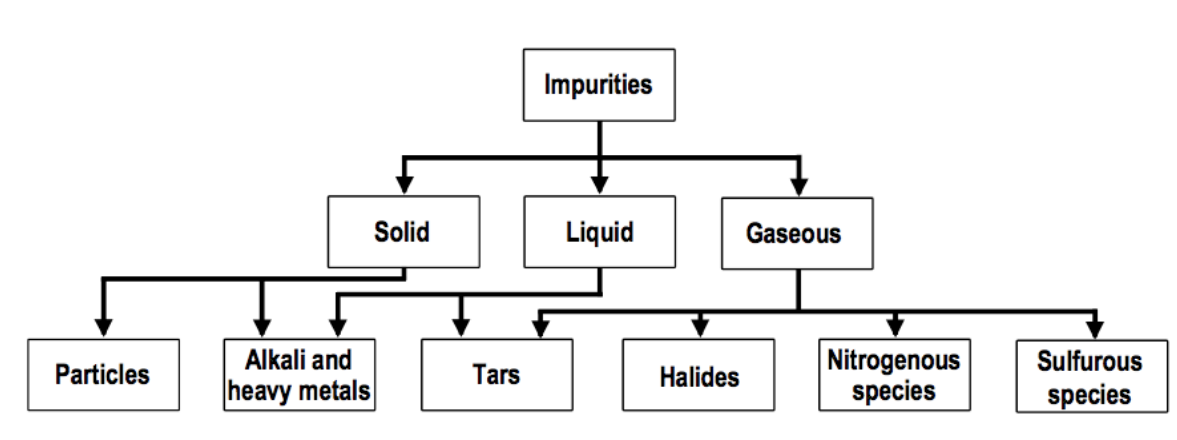
\includegraphics[width=0.5\linewidth]{IMAGES/Renewable/Screenshot from 2025-04-15 23-24-53.png}
\end{figure}

Gas cleaning : \begin{itemize}
    \item PM : scrubbing (<100$^\circ C$), electrostatic precipitation, cyclione, filter
    \item Alkali and halides : they condense on PM
    \item Tars : condense $<100^\circ C$, they can be decomposed thermally or catalytically
    \item Sulphurs : thermally cracked to $H_2S$.
\end{itemize}

\subsubsection{Biogases}
Sources are essentially wet wastes, too inefficient to burn. \\
Waste disposal scheme options : incineration (solid wastes), composting (aerobic, for farming), methanisation (anaerobic digestion), landfill (as a lesser option, when none of the other). 

Anaerobic digestion : transformation of organic matter by microorganisms (bacteria) in absence of $O_2$. Internal reduction + oxidation breakdown of the biomass polymers to the simplest building blocks. Mature technology. AS is a slow process, occurring at room temperature. \\
4 distinct steps : \begin{itemize}
    \item Hydrolysis : slowest of all, breaks solid org. matter down to liquefied monomers and dimers
    \item Digestion : formation of organic acids
    \item Acidogenesis : higher acids break down to $CH_3 COOH$, $H_2$ and $CO_2$
    \item Mathanogenesis : $2CH_3COOH \rightarrow 2CH_4\: +2CO_2$ (70-80\% of $CH_4$ product) and $CO_2+4H_2 \rightarrow CH_4 + 2H_2O$ (20-30\% of $CH_4$ product). Both reactions take place upon different bacterial actions. 
\end{itemize}

Chemical formulas for biogas generation : \begin{itemize}
    \item Buswell formula : $C_aH_b O_c + [a-\frac{1}{4} b-\frac{1}{2} c] H_2O \rightarrow (\frac{1}{2}a + \frac{1}{8}b - \frac{1}{4}c) CH_4 + (\frac{1}{2}a-\frac{1}{8}b + \frac{1}{4}c) CO_2$
    \item Buswell-Boyle : $C_aH_b O_c N_d S_e + \frac{1}{4}[4a- b- 2c + 3d + 2e] H_2O \rightarrow \frac{1}{8}(4a + b - 2c -3d -2e) CH_4 + \frac{1}{8}(4a-b + 2c +3d + 2e) CO_2 + dNH_3 + eH_2S$
\end{itemize}

Digestion is a batch process. mean residence time (days) : $\theta = \frac{V_{reactor}[m^3]}{\dot{V}_{ord}[m^3/d]}$. Daily specific load ($kg/m^3d$) : $M_{day} = \dot{V}_{org} \frac{M}{V} = \frac{M}{\theta}$.\\
Desulfurisation of the biogas is done with $FeCl_3$ solution. Sulfur is removed as it is poisonous. \\
There are 2 main ways to valorise biogas as fuel : separate $CH_4$ from $CO_2$ and inject the $CH_4$ into the NG grid (8\% of use), burn the biogas into a large engine to generate electricity and heat ($92\%$ of use). \\
The current use technologies of biomethane injection and CHP engines impose a scale of biogas production in large digesters to generate biogas flows of 100-1000$m^3/h$. Then, small-scale biogas generate remains unused. \\
It is not sensical to transport a few tonnes of biowaste over more than 5-10km.\\

Bio-electrical systems (BES) : the biological methanation of $CO_2$ is electrocatalyzed in a single step at ambient T and P, using microbes as renewable catalyst. \\

\subsubsection{Liquids}
Advantages : natural resource (reduces oil import), known and simple technology, small plants. Disadvantages : production and substitution (for oil) are limited, requires important infrastructure. \\


\end{document}